\documentclass[italian,12pt,a4paper]{article}
\usepackage[utf8]{inputenc}
\usepackage[T1]{fontenc}
\usepackage{mathtools}
\usepackage{blkarray, bigstrut} %
\usepackage{babel}
\usepackage{graphicx}
\usepackage{subfig}
\usepackage{hyperref}
\usepackage{tikz}
\usepackage{colortbl}
\usepackage{pgf-pie}
\usepackage{algorithm}
\usepackage{algpseudocode}
\usepackage{algorithmicx}
\usepackage{placeins}
\usepackage{tabularx}
\title{Università degli studi di Bari facoltà di scienze MM.FF.NN}
\date{} % clear date
\hypersetup{
	colorlinks=true,
	linkcolor=black,
	filecolor=magenta,      
	urlcolor=cyan,
	pdfpagemode=FullScreen,
}
\graphicspath{ {./img/} }
\RequirePackage[subfigure]{tocloft}

\cftsetindents{section}{0em}{2em}
\cftsetindents{subsection}{0em}{2em}

\usepackage{geometry}
\usepackage{array}
\usepackage{multirow}



\setcounter{tocdepth}{2}
\begin{document}
	\maketitle
	\thispagestyle{empty}
	\begin{center}
		\huge	\textbf{Progetto Metodi Avanzati di Programmazione} \\
		\vspace{20px}
		\Large \textbf{Phosphorus textual-adventure}
	\end{center}
	
	\begin{center}
		by \\
		\Large \textbf{Vito Proscia mat. 735975} \\
	\end{center}
	\vspace{5px}
	\begin{center}
		Email: \href{mailto:v.proscia3@studenti.uniba.it}{v.proscia3@studenti.uniba.it}
	\end{center}
	\vspace{30px}
	\begin{figure}[hb]
		\centering
		
\includegraphics[width=5cm]{image.png}
	\end{figure}
	\vspace{50px}
	\begin{center}
		Repository github: \href{https://github.com/Giut0/Phosphorus-textual-adventure}{Phosphorus}
	\end{center}
	
	\vfill
	\begin{center}
		Anno accadenico 2022-2023
	\end{center}
	
	\newpage
	
	\tableofcontents
	
	\newpage
	
	\section{Introduzione}
	\subsection{Definizione obiettivo principale}
	L'obiettivo principale del progetto è la realizzazione di un'avventura testuale in Java, inglobando, in essa, le tecniche e gli argomenti trattati durante il corso di Metodi Avanzati di Programmazione.
	\subsection{Trama}
		Il protagonista, l’agente f24, si trova su di una navicella spaziale di ritorno alla Terra da una missione che ha consistito nel catturare alieni per produrre il fosforo necessario alla sopravvivenza del pianeta, infatti, sulla quest'ultimo, il fosforo, che riveste un ruolo fondamentale per la sopravvivenza dei vegetali e quindi per il sostentamento dell’uomo è cominciato a diminuire drasticamente, per questo si organizzano spedizioni per catturare alieni in grado di produrlo. \\
		\linebreak
		Inizialmente, f24 si sveglierà dal sonno criogenico nel dormitorio con un ordine, impartito dal comandante, di indagare sulla misteriosa scomparsa di due alieni prigionieri. Il protagonista cercherà i due fuggitivi, districandosi tra le stanze dell’astronave ed interrogando i membri dell’equipaggio, fino a scoprire cosa viene fatto agli alieni prigionieri. Sarà solo a lui decidere se mantenere lo \textit{status quo} o ribellarsi.
	\subsection{Soluzione gioco}
	
		La stanza iniziale è il dormitorio, la prima cosa che si deve fare è prendere la bombola d'ossigeno che sarà utile più avanti, una volta parlato con l'agante a13 bisogna recarsi alla sala meeting, a nord del dormitorio, dopo aver ascoltato il comandante si dovrà prendere la pistola e ci si recherà ad ovest per la mensa, lì ci saranno due scienziati s56 e s99, per proseguire ci si dovrà spostare ad est verso la sala macchine, una volta dentro ci si imbatterà nel primo nemico, l'alieno Orionix, una volta sconfitto bisogneà prendere la chiave dello sgabuzzino, dopo di chè ci si dovrà entrare andando a sud, una volta all'interno si dovrà prendere il bigliettio che conterrà il codice per accedere al laboratorio (4815) che si troverà appena a nord della sala meeting, una volta entrati troveremo l'ultimo nemico Nebulor, che sarà protetto da un altro scienziato, s47, una volta parlato con quest'ultimo starà al giocatore decidere se eliminare l'ultimo nemico o prendere la modifica delle pistola per cercare di cambiare la situazione.
		
		\subsection{Mappa di gioco}
		
		\begin{figure}[!h]
			\centering
			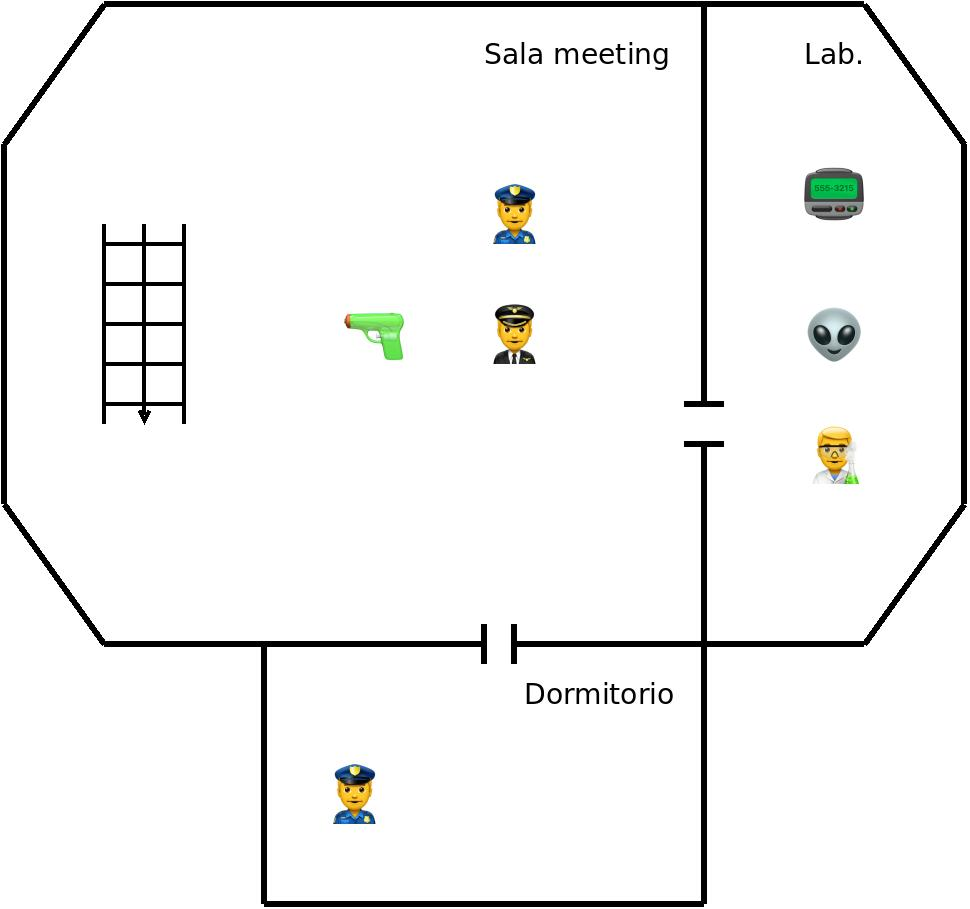
\includegraphics[width=8.5cm]{map1.jpeg}
			\caption{Mappa primo piano}
			\label{fig:mappa_1}
		\end{figure}
		
		\begin{figure}[!h]
			\centering
			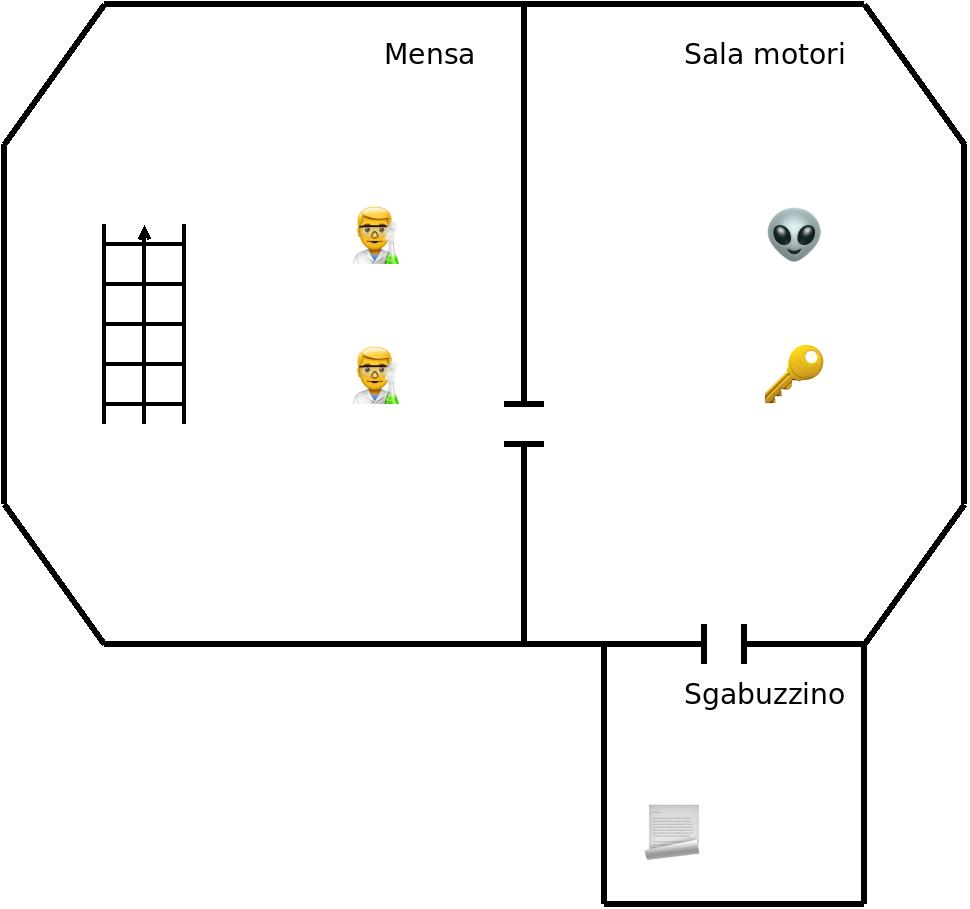
\includegraphics[width=8.5cm]{map2.jpeg}
			\caption{Mappa secondo piano}
			\label{fig:mappa_2}
		\end{figure}
		

\section{Dettagli implementativi}
	In questa sezione verranno analizzate tutte le tecniche e gli argomenti del corso sfruttati per la realizzazione dell'avventura testuale.
	
	\subsection{Progettazione Object-Oriented}
	
	La progettazione orientata agli oggetti (OOD) è un paradigma di programmazione che utilizza "oggetti" come unità fondamentali per progettare, organizzare ed implementare software. Gli oggetti sono istanze di classi cioè astrazioni che rappresentano concetti, dati e operazioni associati al dominio del problema che si sta affrontando, questa metodologia di progettazione garantisce riutilizzabilità del codice, facilità di manutenzione, chiarezza nel flusso di controllo e scalabilità.\\
	\linebreak
	Nello specifico si sono andate a progettare e realizzare una serie di classi garantendo l'incapsulamento di dati e operazioni, di modo che l'accesso a quest'ultimi sia limitato ai metodi della stessa classe, il che promuove la sicurezza e la modularità del codice.\\
	\linebreak
	Al fine di chiarire la struttura delle classi e delle loro relazioni, si è utilizzato il linguaggio di modellazione UML (Unified Modeling Language) per rappresentare in modo visuale la progettazione del software in modo chiaro e conciso.\\
	\linebreak
	Il diagramma delle classi è presente al seguente link: \href{https://github.com/Giut0/Phosphorus-textual-adventure/blob/main/docs/img/class_diagram.jpeg}{class\_diagram\_uml}
	
	\subsection{File}
	Nel progetto i file sono stati utilizzati per modellare gli elementi narrativi e non, dell'avventura, in particolare si hanno a disposizione tre file JSON (JavaScript Object Notation) che vanno a descrivere le stanze, i personaggi e gli oggetti di gioco in modo che le informazioni legate a questi siano facilmente modificabili ed estendibili per migliorare l'avventura, magari aggiungendo più stanze, modificando i dialoghi dei personaggi e perfino stravolgere la trama di gioco. \\
	\linebreak
	All'avvio del gioco avviene la lettura di questi file per inizializzare tutti i vari oggetti che costituiscono l'avventura, questo avviene utilizzando la libreria \href{https://github.com/FasterXML/jackson}{jackson}, che permette di leggere e di utilizzare facilmente i file di tipo JSON, convertendoli in una mappa chiave-valore.
	
	
	\begin{figure}
		\centering
		\subfloat[File delle stanze]{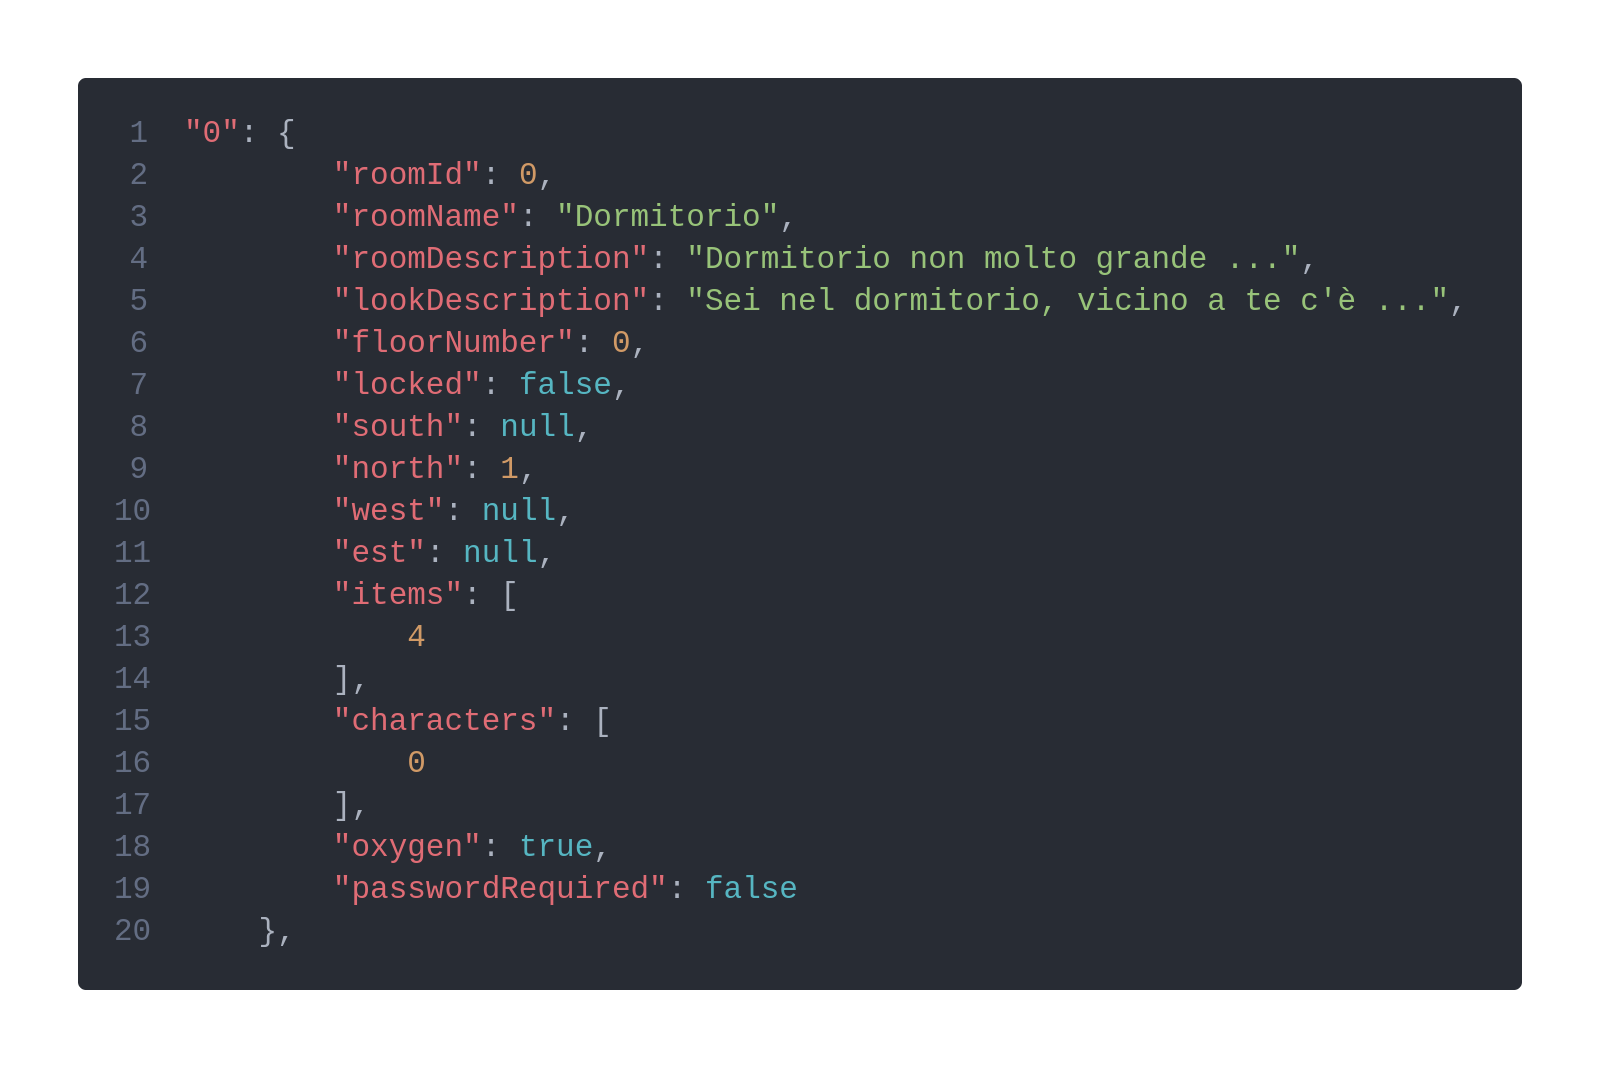
\includegraphics[width=12cm]{code_file1}\label{fig:immagine1}} 
		\\
		\subfloat[File dei personaggi]{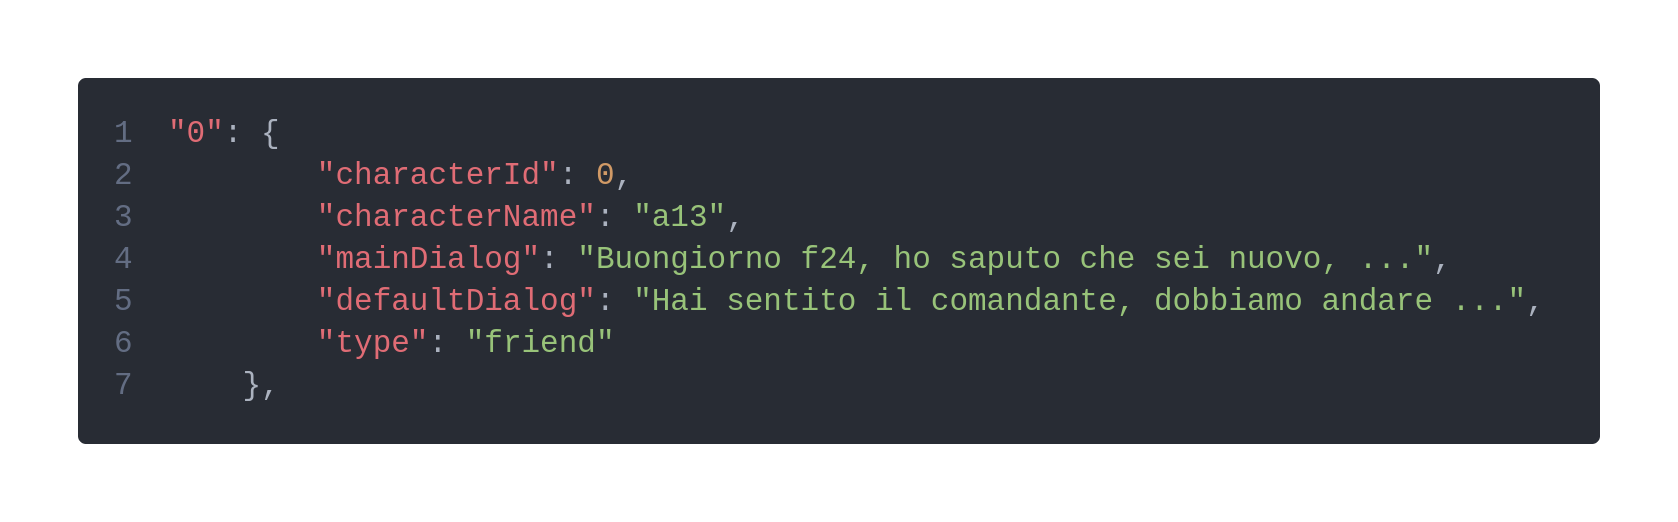
\includegraphics[width=11cm]{code_file2}\label{fig:immagine2}}
		\\
		\subfloat[File degli oggetti di gioco]{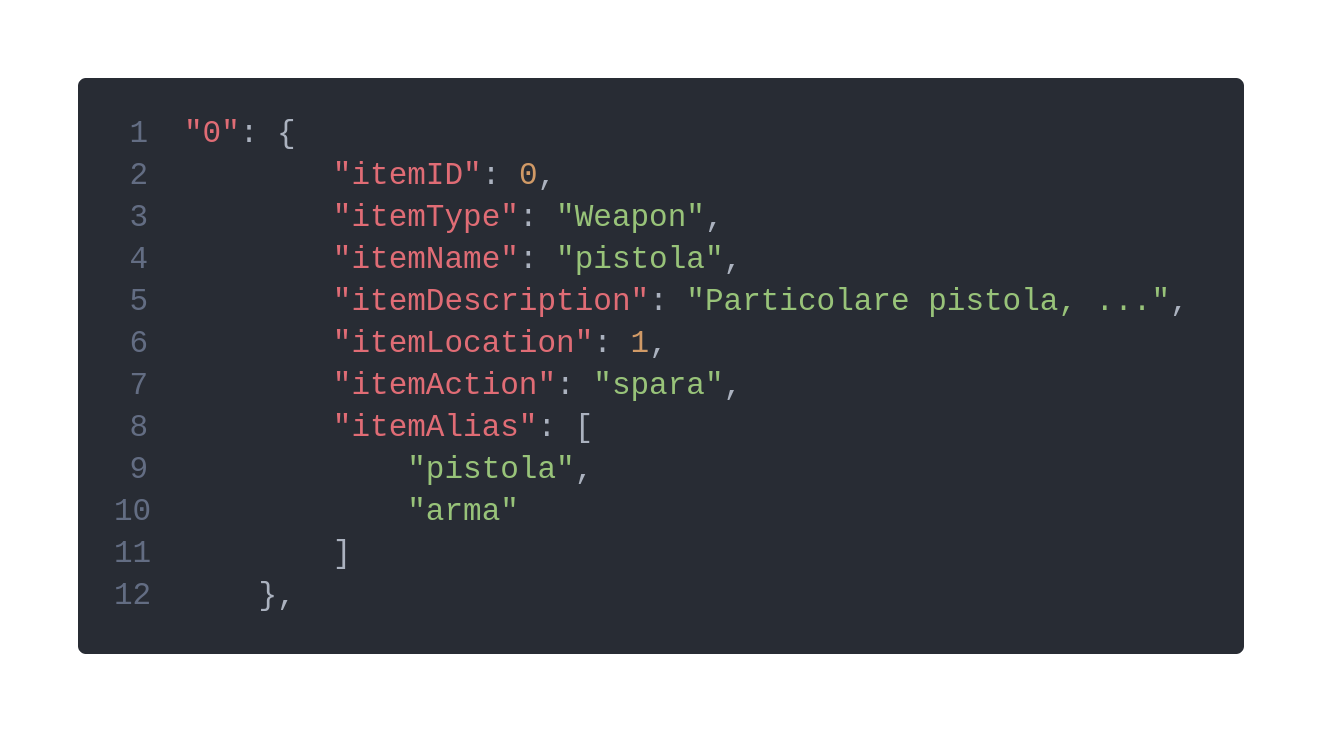
\includegraphics[width=11cm]{code_file3}\label{fig:immagine3}}
		\label{fig:immagini}
	\end{figure}
	
	\subsection{Database}
	
	I salvataggi di gioco sono stati gestiti mediante l'uso delle basi di dati utilizzando JDBC (Java Database Connectivity), in particolare sono state progettate tre relazioni:
	
	\begin{itemize}
		\item game: memorizza i dati relativi al giocatore, come l'id, la stanza in cui si trova, il numero di nemici eliminati ed il timestamp del salvataggio;
		\item inventory: raccoglie tutti gli oggetti recuperati durante l'avventura;
		\item killedCharacter: conserva i dati relativi ai personaggi eliminati nel corso dell'avventura.
	\end{itemize}
	Ogni qual volta che viene salvata la partita, se si esegue il primo salvataggio viene creato il database con le sue relazioni per poi inserire i relativi dati, altrimenti con il nuovo salvataggio vengono sovrascritti i dati del vecchio.\\
	\linebreak
	Si è pensato di sovrascrivere sempre il salvataggio per motivi di semplicità, ma con l'attuale sistema è possibile modificare quest'aspetto dando la scelta al giocatore di salvare/caricare più sessioni.\\
	\linebreak
	Esempio:
	\begin{figure}[!h]
		\centering
		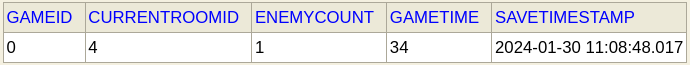
\includegraphics[width=13cm]{db_game.png}
		\caption{Relazione game}
		\label{fig:screen_db1}
	\end{figure}
	\begin{figure}[!h]
		\centering
		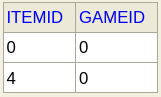
\includegraphics[width=3.5cm]{db_inv.png}
		\caption{Relazione inventory}
		\label{fig:screen_db2}
	\end{figure}
	\begin{figure}[!h]
		\centering
		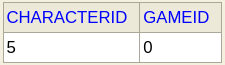
\includegraphics[width=4cm]{db_char.png}
		\caption{Relazione killedCharacter}
		\label{fig:screen_db3}
	\end{figure}
	
	\subsection{Threads}
	I Thread sono unità di esecuzione meno complesse dei processi, essi consentono ad un programma di eseguire più operazioni in modo concorrente, migliorando l'efficienza e consentendo l'esecuzione simultanea di diverse attività. \\
	Per il progetto i thread non stati usati per due scopi differenti:
	
	\begin{enumerate}
		\item \texttt{di.uniba.map.game.GameTimer}: per scandire il tempo di gioco;
		\item \texttt{di.uniba.map.App}: per la riproduzione della musica in sottofondo durante l'esecuzione del gioco, per ulteriori dettagli sulla composizione e produzione della musica, consultare l'Appendice~\ref{appendix:musica}.
	\end{enumerate}
	
	\subsection{Api REST}
	Le API RESTful (Representational State Transfer) sono un'architettura di comunicazione stateless basata su standard web che utilizza metodi HTTP standard, ogni risorsa è unica e raggiungibile attraverso URI  (Uniform Resource Identifier).
	Nel nostro caso le API sono state utilizzate per recuperare le informazioni relative alla qualità dell'aria della città di Bari (41.12° N, 16.86° E) quali:

		\begin{itemize}
			\item European AQI: indice europeo della qualità dell'aria; 
			\item UV index: livello di radiazione UV solare sulla superficie terrestre;
			\item Ozone $O_3$: quantità di ozono nella stratosfera;
			\item Sulphur dioxide $SO_2$: quantità del gas nocivo diossido di zolfo nell'ambiente;
			\item Nitrogen dioxide $NO_2$: quantità del gas nocivo diossido di azoto nell'ambiente;
			
		\end{itemize}
	Si è scelto di reprerire questi valori per una maggiore immersività nella'avventura.\\
	Esempio:
	\begin{figure}[!h]
		\centering
		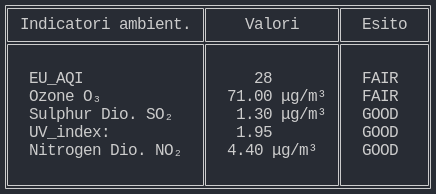
\includegraphics[width=7.5cm]{screen_api}
		\caption{Risultato della chiamata API con valutazione}
		\label{fig:screenapi}
	\end{figure}
	
	\subsection{Java Swing}
	
	Java Swing è un toolkit grafico incluso nella libreria standard di Java per la creazione di interfacce utente (UI) per applicazioni desktop.\\
	Il framework è stato utilizzato per la creazione di un tastierino numerico con i tasti cliccabili (keypad) usato per accedere al laboratorio inserendo la giusta password.
	
	\begin{figure}[!h]
		\centering
		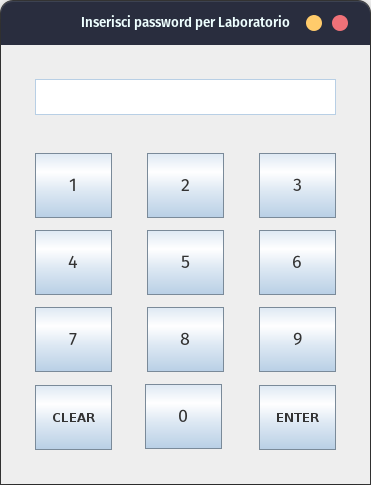
\includegraphics[width=7cm]{screen_keypad}
		\caption{Interfaccia grafica keypad}
		\label{fig:screen_key}
	\end{figure}
	
	
	\begin{figure}
		\centering
		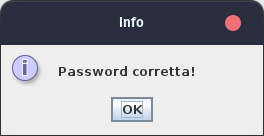
\includegraphics[width=6cm]{screen_corr}\hspace{1cm}
		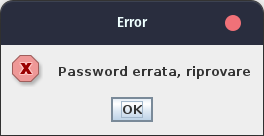
\includegraphics[width=6cm]{screen_err}
		\caption{Messaggi in caso di risposta corretta/errata}
		\label{fig:screen_allineate}
	\end{figure}
	
	\section{Sommario classi implementate}
	In questa sezione sarà presentata una breve panoramica delle classi implementate nel progetto.
	
	\subsection{\texttt{di.uniba.map}}
		In questo package sono contenute la classi principali per l'avvio del gioco:
		
		\begin{itemize}
			\item App: classe che fa partire il gioco, contiene il metodo \textit{main};
			\item Utils: classe contenente tutti i vari metodi di supporto alle altre classi del progetto.
		\end{itemize}
	
	\subsection{\texttt{di.uniba.map.game}}
		Nucleo centrale del progetto, questo package ingloba tutte le classi necessarie al funzionamento del gioco collegando le altre classi insieme:
		
		\begin{itemize}
			\item AirQuality: classe che si occupa di gestire la chiamata API al servizio di \href{https://open-meteo.com/en/docs/air-quality-api}{open-meteo};
			\item GameEngine: classe che regola lo scheletro di gioco inglobando tutte le varie azioni effettuabili, le stanze disponibili, l'inventario e la stanza corrente;
			\item GameTimer: si occupa dell'esecuzione del thread timer;
			\item PhosphorusGame: gestisce le varie azioni disponibili, sia del menù che del gioco vero e proprio;
			\item SaveGame: classe che coordina i salvataggi di gioco, contiene i metodi per salvare e riprendere la sessione di gioco.
		\end{itemize}
		
	
	\subsection{\texttt{di.uniba.map.parser}}
	Le classi all'interno di questo package gestiscono l'input del giocatore convertendolo in azioni di gioco:
	\begin{itemize}
		\item Parser: classe che analizza l'input del giocatore cercando di meglio interpretalo per convertire il tutto in azioni di gioco (azione, azione-oggetto e azione-personaggio);
		\item ParserOutput: classe che compone il comando che il giocatre impartisce.
	\end{itemize}
	
	\subsection{\texttt{di.uniba.map.type}}
	Questo package contiene tutti i tipi progettati che compongono il gioco:
	\begin{itemize}
		\item Action: rappresenta le azioni di gioco;
		\item ActionType: contiene tutte le tipologie di azioni;
		\item Character: descrive le caratteristiche dei personaggi di gioco;
		\item Enemy: specializzazione della classe Character che gestisce le informazioni dei nemici;
		\item Inventory: rappresenta l'inventario di gioco; 
		\item Item: descrive un oggetto di gioco;
		\item KetItem: specializzazione di Item per rappresentare gli oggetti chiave;
		\item Room: rappresenta le stanze le compongono il gioco;
		\item Weapon: specializzazione della classe Item, rappresenta gli oggetti che possono danneggiare i personaggi.
	\end{itemize}
	
	\subsection{\texttt{di.uniba.map.ui}}
	Le classi contenutevi compongono l'interfaccia utente del gioco: 
	\begin{itemize}
		\item JKeypad: classe che gestisce la GUI (Graphical User Interface) del tastierino numerico utile ad accedere al laboratorio andando ad inserire una passowrd;
		\item UI: contiene tutti i metodi relativi alla stampa a schermo delle varie componenti del gioco, quali la mappa, il menù, i vari finali, etc\dots.
	\end{itemize}
	\section{Conclusioni}
	
	In conclusione, l'obiettivo principale del progetto è stato lo sviluppo di un'avventura testuale in Java, mettendo insieme tutte le tecniche studiate durate il corso M.A.P. con la possibilità di aggiungere creatività per legare il tutto.\\
	\linebreak
	Personalmente mi ritengo soddisfatto del risultato finale, sia in termini di progettazione che di realizzazione, il tutto mi ha permesso di migliorare assimilando il paradigma di programmazione ad oggetti, donandomi un nuova \textit{forma mentis} che sicuramente mi aiuterà ad affrontare ed a risolvere problemi futuri. 

	\section{Sviluppi futuri}
	
	Nonostante il raggiungimento degli obiettivi preposti il progetto è aperto a sviluppi futuri che possono migliorare l'esperienza dei giocatori, eccone alcuni esempi:
	
	\begin{enumerate}
		\item Implementazione di una vera e propria GUI;
		\item Possibilità di creare/caricare più salvataggi;
		\item Aggiunta di componenti queli il livello di salute del giocatore e dei nemici, con possibilità di far attaccare quest'ultimi.
	\end{enumerate}
	Queste sono alcune delle idee da implementare per rendere il gioco più accattivante e divertente.
	
	\appendix
	\section{Musica}\label{appendix:musica}
	In questa sezione appendice verranno presentati tutti gli step della creazione della colonna sonora di gioco "short\_circuit" che ho realizzato per migliorare l'esperienza del giocatore, mettendo a frutto la mia grande passione per la musica.
	
	\subsection{Composizione}
	Per arricchire l'atmosfera ho incluso nel progetto una mia improvvisazione musicale, cercando di trasmettere un po' quel senso di mistero che avvolge la vicenda di gioco, al fine di far immergere il giocatore ancor meglio nell'avventura.
	
	\begin{figure}[!h]
		\centering
		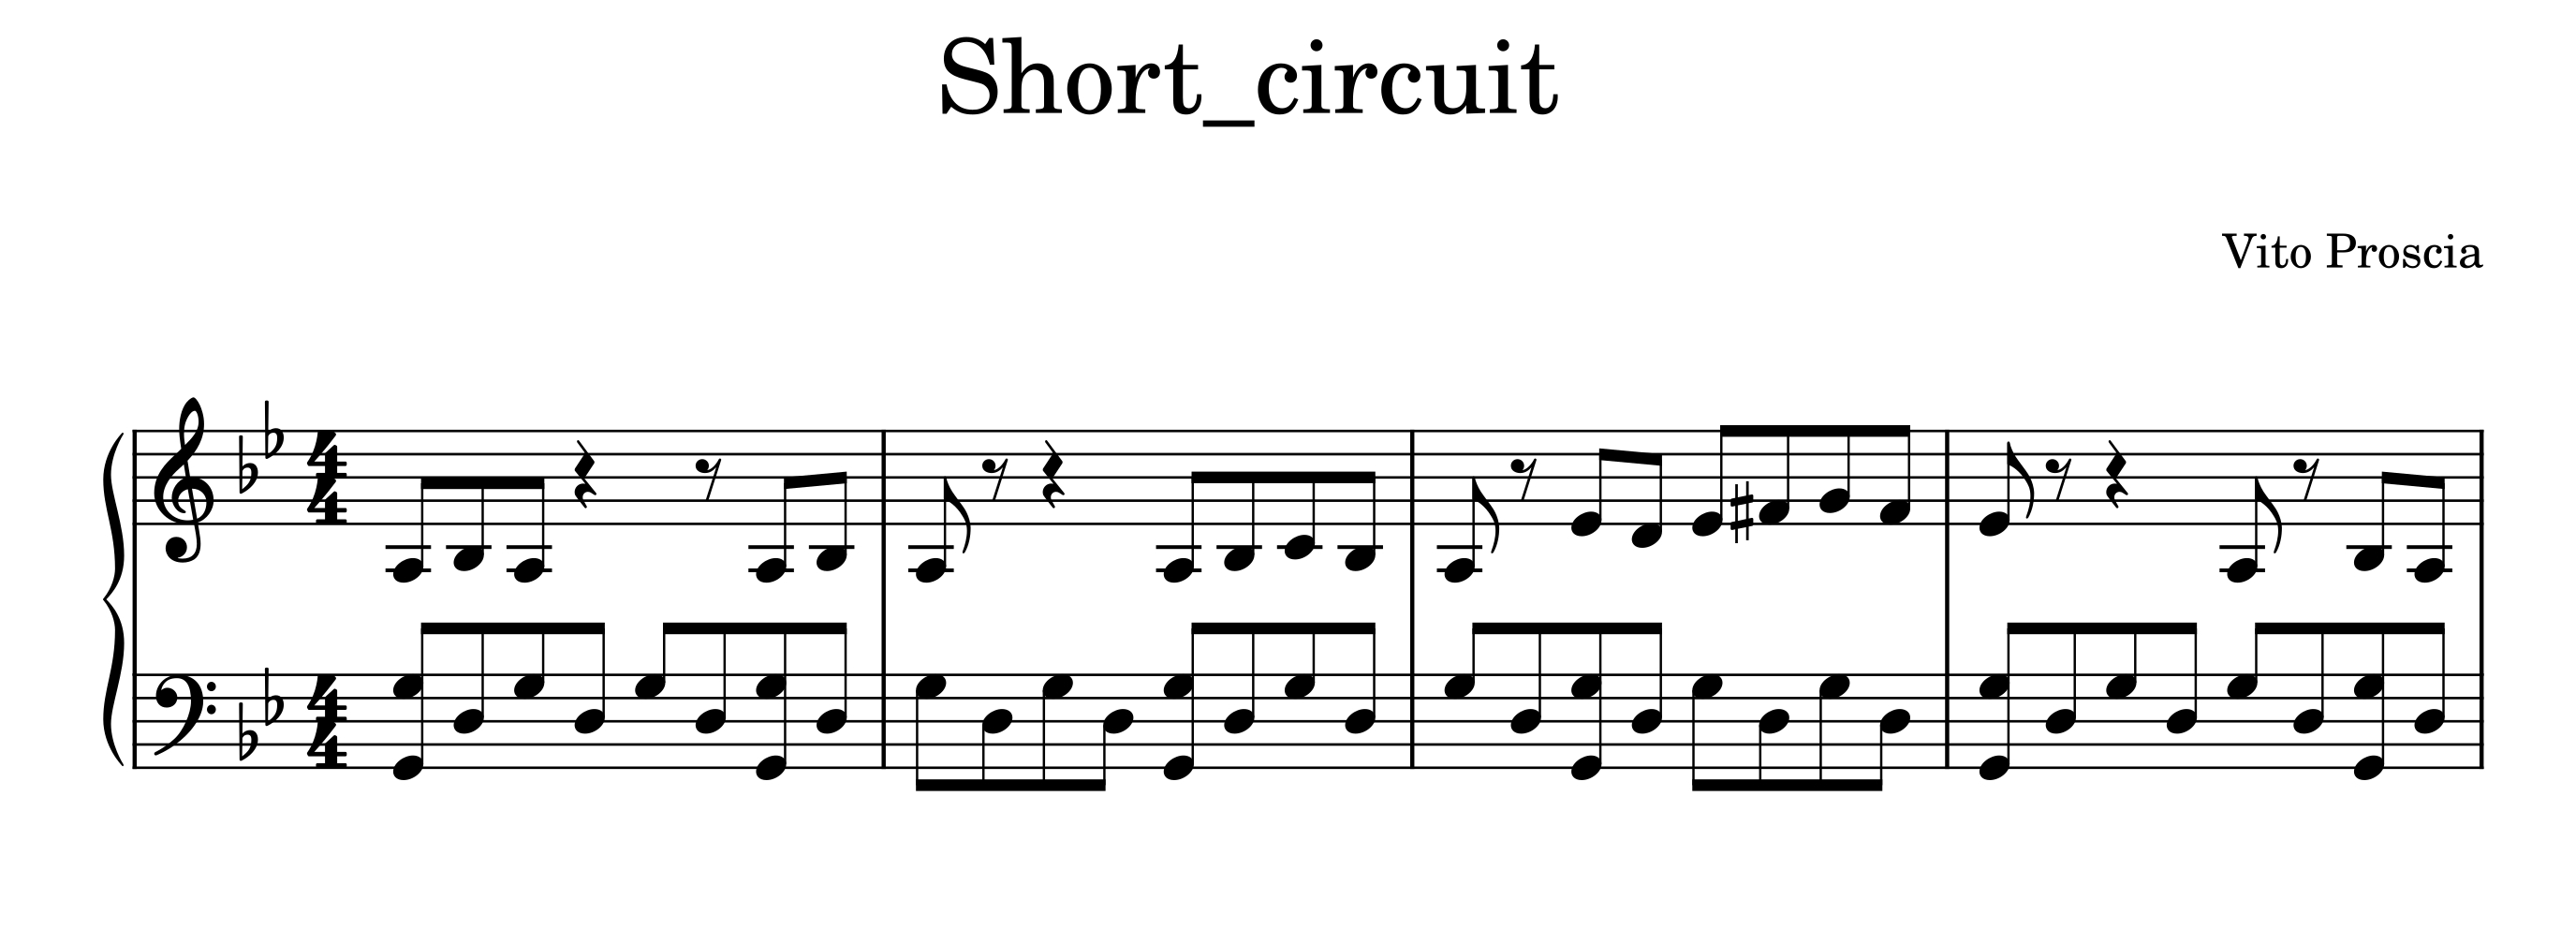
\includegraphics[width=14cm]{score}
		\caption{estratto spartito di "Short\_circuit"}
		\label{fig:score}
	\end{figure}
	
	\subsection{Produzione}
	La parte relativa alla produzione musicale è stata una delle più ardue ed al contempo una delle più divertenti, personalmente non mi ero mai cimentato, fino a questo momento, nella produzione di un brano musicale.\\
	\linebreak
	Nello specifico, con la funzione record del pianoforte digitale, ho registrato il brano per poi salvarlo in formato MIDI (Musical Instrument Digital Interface), successivamente ho esportato il file nell'applicazione per iPad Garageband, che permette, amatorialmente, di creare musica, per poi modificare lo strumento di esecuzione, aggiungere degli effetti sonori come il wabble ed il riverbero ed andare ad editare la traccia audio, tagliando o registrando nuovamente delle parti, infine ho salvato il tutto sotto froma di WAV (Waveform) per poi imporare il brano nel progetto facendo sì che sia riprodotto in loop durante il gioco. \\
	\linebreak
	\begin{figure}[!h]
		\centering
		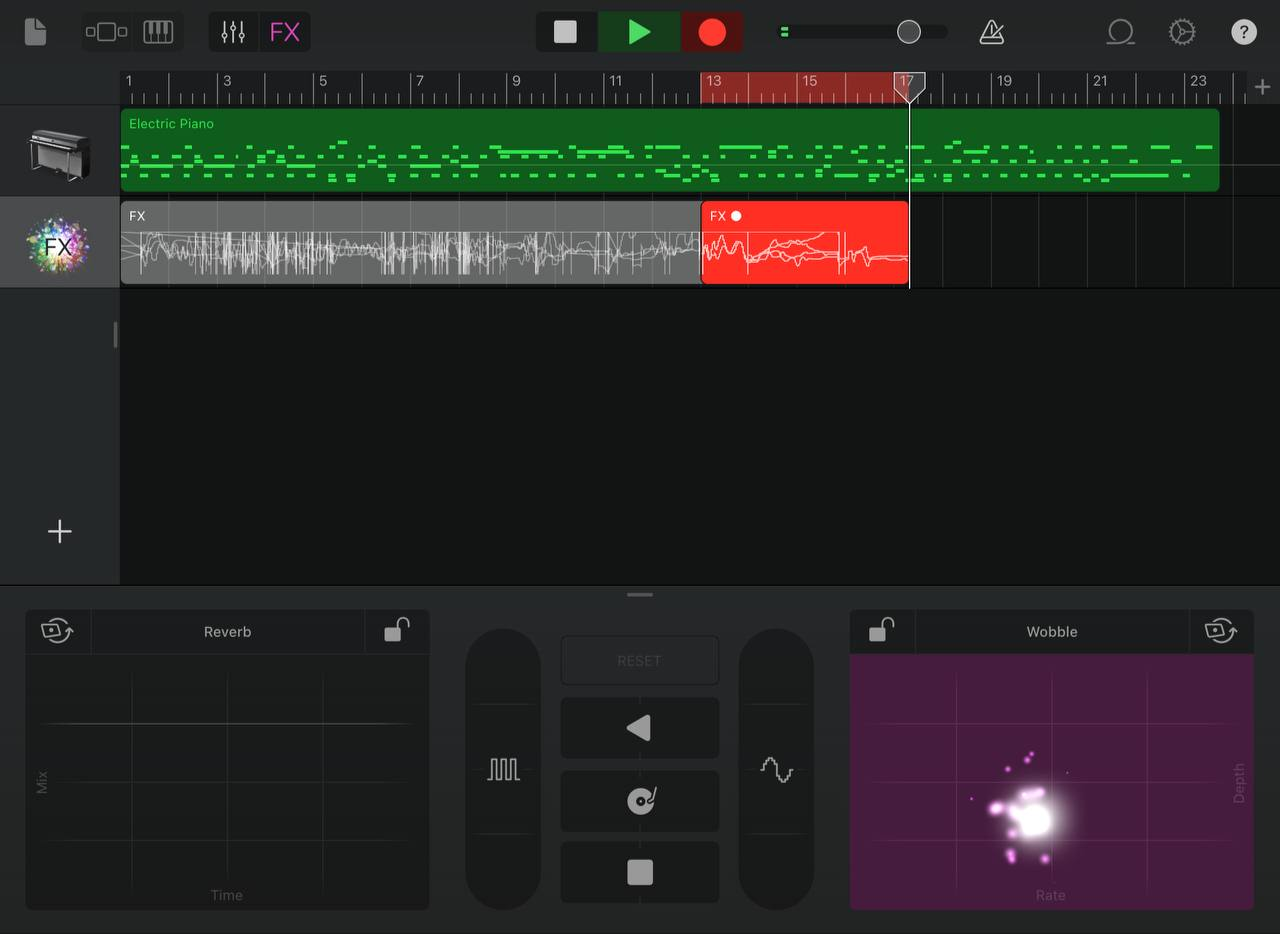
\includegraphics[width=14cm]{garageband.jpg}
		\caption{Screenshot dell'applicazione Garageband}
		\label{fig:musica}
	\end{figure}
	
	\section{Specifica algebrica della Lista}
	In questa sezione appendice verrà presentata la specifica algebrica della struttura dati Lista.
	\subsection{Specifica sintattica}
	
	\textbf{Sorts}: Lista, Elemento, Boolean, Integer, Posizione. \\
	\linebreak
	\textbf{Operations}:
	\begin{itemize}
		\item creaLista() $\rightarrow$ Lista
		\item listaVuota(Lista) $\rightarrow$ Boolean
		\item leggiLista(Lista, Posizione) $\rightarrow$ Elemento
		\item cancLista(Lista, Posizione) $\rightarrow$ Lista
		\item insLista(Lista, Elemento) $\rightarrow$ Lista
		\item lunghezza(Lista) $\rightarrow$ Integer
		\item contiene(Lista, Elemento) $\rightarrow$ Boolean
	\end{itemize}
	
	\subsection{Specifica semantica}
	
	\begin{table}[!ht]
		\centering
		\renewcommand{\arraystretch}{1.5}
		\begin{tabular}{|c|c|c|}
			\hline
			\multirow{2}{*}{Osservatori} & \multicolumn{2}{c|}{Costruttori di $l'$} \\
			\cline{2-3}
			& creaLista() & insLista($l$, $p$, $i$) \\
			\hline
			listaVuota($l'$) & true & false \\
			\hline
			leggiLista($l'$, $p'$) & error & $if$ $p=p'$ $then$ $i$ $else$ leggiLista($l$, $p'$) \\
			\hline
			cancLista($l'$, $p'$) & error & $if$ $p=p'$ $then$ $l$ $else$ insLista(cancLista($l$, $p'$), $p$, $i$) \\
			\hline
			lunghezza($l'$) & 0 & lunghezza($l$) + 1 \\
			\hline
			contiene($l'$, $i'$) & false & $if$ $i=i'$ $then$ true $else$ contiene($l$, $i'$)  \\
			\hline

		\end{tabular}
		\caption{Tabella per la costruzione degli operatori della specifica semantica}
		\label{tab:esempio}
	\end{table}
	\textbf{Declere}:
	\begin{itemize}
		\item $l$ : Lista<Elemento>
		\item $i$ : Elemento
		\item $p$ : Posizione
		\item ${true, false}$ : Boolean
	\end{itemize}
	
	\textbf{Operations}:
	
	\begin{itemize}
		\item listaVuota(creaLista()) $\rightarrow$ true
		\item listaVuota(insLista($l$, $p$, $i$)) $\rightarrow$ false
		
		\item leggiLista(insLista($l$, $p$, $i$), $p'$) $\rightarrow$ $if$ $p=p'$ $then$ $i$ $else$ leggiLista($l$, $p'$)
		
		\item cancLista(insLista($l$, $p$, $i$), $p'$) $\rightarrow$ $if$ $p=p'$ $then$ $l$ $else$ insLista(cancLista($l$, $p'$), $p$, $i$)
		
		\item lunghezza(creaLista()) $\rightarrow$ 0
		\item lunghezza(insLista($l$, $p$, $i$)) $\rightarrow$ lunghezza($l$) + 1
		
		\item contiene(creaLista(), $i'$) $\rightarrow$ false
		\item contiene(insLista($l$, $p$, $i$), $i'$) $\rightarrow$ $if$ $i=i'$ $then$ true $else$ contiene($l$, $i'$)
	\end{itemize}
	
	\subsection{Specifica di restrizione}
	
	\begin{itemize}
		\item leggiLista(creaLista(), $p'$) $\rightarrow$ error
		\item cancLista(creaLista(), $p'$) $\rightarrow$ error
	\end{itemize}
	
\end{document}